\documentclass[a0,portrait]{a0poster}

\usepackage{multicol}
\columnsep=100pt
\columnseprule=3pt

\usepackage[svgnames]{xcolor}

\usepackage{times}
\usepackage{palatino}
\usepackage[none]{hyphenat}
\usepackage{graphicx}
\graphicspath{{figures/}}
\usepackage{booktabs}
\usepackage[font=small,labelfont=bf]{caption}
\usepackage{amsfonts, amsmath, amsthm, amssymb}
\usepackage{wrapfig}
\usepackage{lipsum,adjustbox}
\usepackage[absolute,overlay]{textpos}
\usepackage{multirow}
\usepackage{titlesec}
\usepackage[inline]{enumitem}
\usepackage{url}
\usepackage{tikz,pgfplots,pgfplotstable}
\usepackage{tikz-dependency}
\usetikzlibrary{arrows.meta}
\captionsetup{labelformat=empty}

\begin{document}

\begin{center}
	\veryHuge \color{NavyBlue} \textbf{Multitask Parsing Across Semantic Representations}
\end{center}
\vspace{-1cm}
\begin{minipage}[b]{.07\linewidth}

\includegraphics[width=\linewidth]{huji_logo.jpg}
\vspace{5mm}
\end{minipage}
\begin{minipage}[b]{.16\linewidth}

\includegraphics[width=\linewidth]{huji_banner.png}

\includegraphics[width=\linewidth]{cse_banner.jpg}
\vspace{.8mm}
\end{minipage}
\hspace{1cm}
\begin{minipage}[b]{0.57\linewidth}
\LARGE \textbf{Daniel Hershcovich}\textsuperscript{1,2} \&
	   \textbf{Omri Abend}\textsuperscript{2} \&
	   \textbf{Ari Rappoport}\textsuperscript{2} \\[0.5cm]
\Large $^1$The Edmond and Lily Safra Center for Brain Sciences \\
  $^2$School of Computer Science and Engineering
  \setlength{\columnseprule}{0pt}
  \setlength\multicolsep{-20pt}
  \begin{multicols}{2}
  The Hebrew University of Jerusalem
  \large \texttt{\{danielh,oabend,arir\}@cs.huji.ac.il}
  \end{multicols}
\end{minipage}
\hfill
\begin{minipage}[b]{.09\linewidth}

\includegraphics[width=\linewidth]{elsc_logo.png}\vspace{5mm}

\includegraphics[width=\linewidth]{icrici_banner.png}
\end{minipage}

\vspace{1cm}
\titlespacing*{\section}{0pt}{8mm}{5mm}

%----------------------------------------------------------------------------------------

\begin{adjustbox}{margin=3mm,frame,minipage=.6\linewidth,center}
\Large\color{Navy}
Multitask learning allows a transition-based semantic parser
to generalize from multiple tasks,
improving UCCA parsing in challenging settings.
\end{adjustbox}


\begin{multicols}{2}


\color{Black}

\section*{Introduction}

Semantic parsing is important for natural language understanding.
Representation schemes vary,
but data is mostly \textbf{small}, \textbf{in-domain}, and in \textbf{English}.
\hfill We consider four schemes:
\begin{itemize}[nosep,labelsep=1em]
{\color{Indigo} \item[\textbf{UCCA}:] Intuitive, cross-lingual, and modular semantic representation.
    \textit{Primary edges} form a tree. \textit{Remote edges} (dashed) allow reentrancy,
    creating a directed acyclic graph (DAG).
    Edge labels encode predicate-argument structure, semantic heads and inter-scene relations
    \cite{abend2013universal}.}
{\color{DarkGreen} \item[\textbf{AMR}:] Abstract graph on concepts and constants.
    Rooted DAG with labeled nodes and edges.
    Encodes named entities, argument structure, semantic roles, word sense, coreference \cite{banarescu2013abstract}.}
{\color{DarkRed} \item[\textbf{SDP}:] Set of related bilexical semantic DAG schemes (DM, PAS, PSD and CCD).
    We use \textbf{DM}~(DELPH-IN~MRS).
    Encodes argument structure for many predicate types \cite{oepen2016towards}.}
{\color{DarkBlue} \item[\textbf{UD}:] Cross-lingual syntactic bilexical tree.
    Encodes syntactic relations between words \cite{nivre2016universal}. \\
    \textbf{UD$^{++}$} (Enhanced++ UD) adds and augments edges, creating a bilexical DAG
    \cite{SCHUSTER16.779}.}
\end{itemize}

\begin{minipage}{.8\columnwidth}
  \color{Indigo}
  \begin{center}
    \begin{tikzpicture}[level distance=3cm, sibling distance=55mm, -{Latex[length=5mm]},
        every node/.append style={font=\bf\ttfamily},
        every circle node/.append style={fill=Indigo}]
      \tikzstyle{word} = [font=\rmfamily,color=black]
      \node (ROOT) [circle] {}
        child {node (After) [word] {After} edge from parent node[above] {L}}
        child {node (graduation) [circle] {}
        {
          child {node [word] {graduation} edge from parent node[left] {P}}
        } edge from parent node[right] {H} }
        child {node [word] {,} edge from parent node[below] {U}}
        child {node (moved) [circle] {}
        {
          child {node (John) [word] {John} edge from parent node[left] {A}}
          child {node [word] {moved} edge from parent node[left] {P}}
          child {node [circle] {}
          {
            child {node [word] {to} edge from parent node[left] {R}}
            child {node [word] {Paris} edge from parent node[right] {C}}
          } edge from parent node[above] {A} }
        } edge from parent node[above] {H} }
        ;
      \draw[dashed,-{Latex[length=5mm]}] (graduation) to node [above] {A} (John);
    \end{tikzpicture}
  \captionof{figure}{\color{Indigo} Universal Conceptual Cognitive Annotation (UCCA).}
  \end{center}
\end{minipage}
\hfill
\begin{minipage}{.2\columnwidth}
  \begin{center}
  \begin{adjustbox}{margin=2mm,frame,scale=.75}
  \color{Indigo}
  \begin{tabular}{>{\bf\ttfamily}cl}
	  P & process \\
	  S & state \\
	  A & participant \\
	  L & linker \\
	  H & linked scene \\
	  C & center \\
	  E & elaborator \\
	  D & adverbial \\
	  R & relator \\
	  N & connector \\
	  U & punctuation \\
	  F & function unit \\
	  G & ground
  \end{tabular}
  \end{adjustbox}
  \captionof{table}{\color{Indigo} UCCA edge labels.}
  \end{center}
\end{minipage}

\begin{minipage}{.45\columnwidth}
  \begin{center}
  \begin{tikzpicture}[-{Latex[length=5mm]}, color=DarkGreen, level distance=45mm,
      every node/.append style={sloped,anchor=south,auto=false,font=\scriptsize\bf\ttfamily},
      level 1/.style={sibling distance=55mm}]
    \node (ROOT) [draw=DarkGreen,ellipse] {move-01}
      child {node [draw=DarkGreen,ellipse] {after}
      {
            child {node (graduation) [draw=DarkGreen,ellipse] {graduate-01} edge from parent node {op1} }
      } edge from parent node {time} }
      child {node (John) [draw=DarkGreen,ellipse] {person}
      {
        child {node [draw=DarkGreen,ellipse] {name}
        {
            child {node [draw=DarkGreen,ellipse] {"John"} edge from parent node {op1} }
        } edge from parent node {name} }
      } edge from parent node {ARG0} }
      child {node [draw=DarkGreen,ellipse] {city}
      {
        child {node [draw=DarkGreen,ellipse] {name}
        {
            child {node [draw=DarkGreen,ellipse] {"Paris"} edge from parent node {op1} }
        } edge from parent node {name} }
      } edge from parent node {ARG2} }
      ;
      \draw (graduation) to node {ARG0} (John);
  \end{tikzpicture}
  \captionof{figure}{\color{DarkGreen} Abstract Meaning Representation (AMR).}
  \end{center}
\end{minipage}
\begin{minipage}{.55\columnwidth}
    \begin{center}
    \begin{dependency}[edge style={-{Latex[length=4mm]}, color=DarkRed},
        text only label, label style={above, color=DarkRed, font=\bf\ttfamily}, font=\small]
    \begin{deptext}[column sep=.8em,ampersand replacement=\^]
    After \^ graduation \^ , \^ John \^ moved \^ to \^ Paris \\
    \end{deptext}
        \depedge[edge unit distance=1em]{1}{2}{ARG2}
        \depedge[edge unit distance=1em, edge start x offset=-4mm]{5}{4}{ARG1}
        \depedge[edge unit distance=1em, edge end x offset=-3mm]{1}{5}{ARG1}
        \deproot[edge unit distance=1.25em]{5}{top}
        \depedge[edge unit distance=2em, edge start x offset=1mm, edge end x offset=3mm]{5}{7}{ARG2}
        \depedge[edge unit distance=1em, edge end x offset=5mm]{6}{5}{ARG1}
        \depedge[edge unit distance=1em]{6}{7}{ARG2}
    \end{dependency}
    \captionof{figure}{\color{DarkRed} Semantic Dependency Parsing (SDP): DM representation.}
    \vfill
    \begin{dependency}[edge style={-{Latex[length=4mm]}, color=DarkBlue},
        text only label, label style={above, color=DarkBlue, font=\bf\ttfamily}, font=\small]
    \begin{deptext}[column sep=.8em,ampersand replacement=\^]
    After \^ graduation \^ , \^ John \^ moved \^ to \^ Paris \\
    \end{deptext}
        \depedge[edge unit distance=1em]{2}{1}{case}
        \depedge[edge unit distance=1em]{4}{3}{punct}
        \depedge[edge unit distance=1em, edge start x offset=-4mm]{5}{4}{nsubj}
        \depedge[edge unit distance=1em, edge end x offset=-3mm]{2}{5}{obl}
        \depedge[edge unit distance=1em]{7}{6}{case}
        \deproot[edge unit distance=1em]{5}{root}
        \depedge[edge unit distance=1.5em, edge start x offset=1mm]{5}{7}{obl}
    \end{dependency}
  \captionof{figure}{\color{DarkBlue} Universal Dependencies (UD).}
  \end{center}
\end{minipage}

While formally different, semantic representations
share much of their content \cite{abend2017state}.
\textbf{Multitask learning} exploits the overlap between parsing tasks
and effectively extend the training data
for our transition-based DAG parser,
showing benefits for UCCA parsing.


We focus on UCCA due to its small training set,
where multitask learning is likely to help the most.
As auxiliary tasks, we use \textbf{unlabeled} AMR, SDP and UD parsing.

\hrule

\section*{Data}

\begin{itemize*}
\item [\textbf{\color{Indigo} UCCA}:] \color{Indigo} (1) \textbf{English} Wikipedia (\textbf{Wiki});
(2) \textit{Twenty Thousand Leagues Under the Sea} (\textbf{20K}),
annotated in \textbf{English} (small, only test) \textbf{French} (small), and \textbf{German}
(pre-release, noisy).
\item [\textbf{\color{DarkGreen} AMR}:] \color{DarkGreen} LDC2017T10 (\textbf{English}).
\item [\textbf{\color{DarkRed} SDP}:] \color{DarkRed} DM part from SDP 2016 (\textbf{English}).
\item [\textbf{\color{DarkBlue} UD}:] \color{DarkBlue} \textbf{English}, \textbf{French} and \textbf{German} treebanks,
v2.1 (UD$^{++}$ for English).
\end{itemize*}
\hfill Number of sentences per dataset:

\hspace{-35mm}
\begin{minipage}{.4\columnwidth}
\pgfplotstableread[row sep=\\,col sep=&]{
	corpus & train & dev & test \\
	\color{DarkBlue} \textbf{UD} & 17062 & 0 & 0 \\
	\color{DarkRed} \textbf{SDP} & 33964 & 0 & 0 \\
	\color{DarkGreen} \textbf{AMR} & 36521 & 0 & 0 \\
	\color{Indigo} \textbf{Wiki} & 4268 & 454 & 503 \\
	\color{Indigo} \textbf{20K} & 0 & 0 & 506 \\
    }\english
\begin{center}
    \begin{tikzpicture}
    \begin{axis}[
    xbar stacked,
    width=13cm,
    height=9cm,
    xmin=0,
    xmax=70000,
    xtick=\empty,
    ytick=data,
    yticklabels from table={\english}{corpus}
    ]
    \addplot [fill=green!80] table [x=train, meta=corpus,y expr=\coordindex] {\english};
    \addplot [fill=blue!60] table [x=dev, meta=corpus,y expr=\coordindex] {\english};
    \addplot [fill=red!60, point meta=x, nodes near coords, nodes near coords align={anchor=west},
    every node near coord/.append style={
        black,
        fill=white,
        fill opacity=0.75,
        text opacity=1,
        outer sep=\pgflinewidth
    }
    ] table [x=test, meta=corpus,y expr=\coordindex] {\english};
    \end{axis}
    \end{tikzpicture}
    \captionof{figure}{\hspace{35mm} \textbf{English} corpora.}
\end{center}
\end{minipage}
\hspace{1mm}
\begin{minipage}{.34\columnwidth}
\pgfplotstableread[row sep=\\,col sep=&]{
	corpus & train & dev & test \\
	UD & 32347 & 0 & 0 \\
	UCCA 20K & 413 & 67 & 67 \\
    }\french
\begin{center}
    \begin{tikzpicture}
    \begin{axis}[
    xbar stacked,
    width=13cm,
    height=9cm,
    xmin=0,
    xmax=70000,
    xtick=\empty,
    ytick=\empty,
    yticklabels=\empty
    ]
    \addplot [fill=green!80] table [x=train, meta=corpus,y expr=\coordindex] {\french};
    \addplot [fill=blue!60] table [x=dev, meta=corpus,y expr=\coordindex] {\french};
    \addplot [fill=red!60, point meta=x, nodes near coords, nodes near coords align={anchor=west},
    every node near coord/.append style={
        black,
        fill=white,
        fill opacity=0.75,
        text opacity=1,
        outer sep=\pgflinewidth
    }
    ] table [x=test, meta=corpus,y expr=\coordindex] {\french};
    \end{axis}
    \end{tikzpicture}
    \captionof{figure}{\textbf{French} corpora.}
\end{center}
\end{minipage}
\begin{minipage}{.34\columnwidth}
\pgfplotstableread[row sep=\\,col sep=&]{
	corpus & train & dev & test \\
	UD & 13814 & 0 & 0 \\
	UCCA 20K & 3429 & 561 & 2164 \\
    }\german
\begin{center}
    \begin{tikzpicture}
    \begin{axis}[
    xbar stacked,
    width=13cm,
    height=9cm,
    xmin=0,
    xmax=70000,
    xtick=\empty,
    ytick=\empty,
    legend style={at={(axis cs:50000,.8)},anchor=north west},
    yticklabels=\empty
    ]
    \addplot [fill=green!80] table [x=train, meta=corpus,y expr=\coordindex] {\german};
    \addplot [fill=blue!60] table [x=dev, meta=corpus,y expr=\coordindex] {\german};
    \addplot [fill=red!60, point meta=x, nodes near coords, nodes near coords align={anchor=west},
    every node near coord/.append style={
        black,
        fill=white,
        fill opacity=0.75,
        text opacity=1,
        outer sep=\pgflinewidth
    }
    ] table [x=test, meta=corpus,y expr=\coordindex] {\german};
    \legend{train,dev,test}
    \end{axis}
    \end{tikzpicture}
    \captionof{figure}{\textbf{German} corpora.}
\end{center}
\end{minipage}


While UCCA is annotated over Wikipedia and over a literary corpus,
the domains for AMR, SDP and UD are blogs, news, emails, reviews, and Q\&A---a challenging setting.

\hrule


\section*{General Transition-based DAG Parser}

We extend TUPA \cite{hershcovich2017a}, a UCCA parser supporting
reentrancy, discontinuity and non-terminal nodes.
It applies a \textit{transition}
at each step to the parser state, comprising
a working \textbf{stack} of nodes,
\textbf{buffer} of remaining nodes and tokens,
and \textbf{graph} of constructed nodes and edges.

\scalebox{.9}{
\begin{minipage}{.55\columnwidth}
	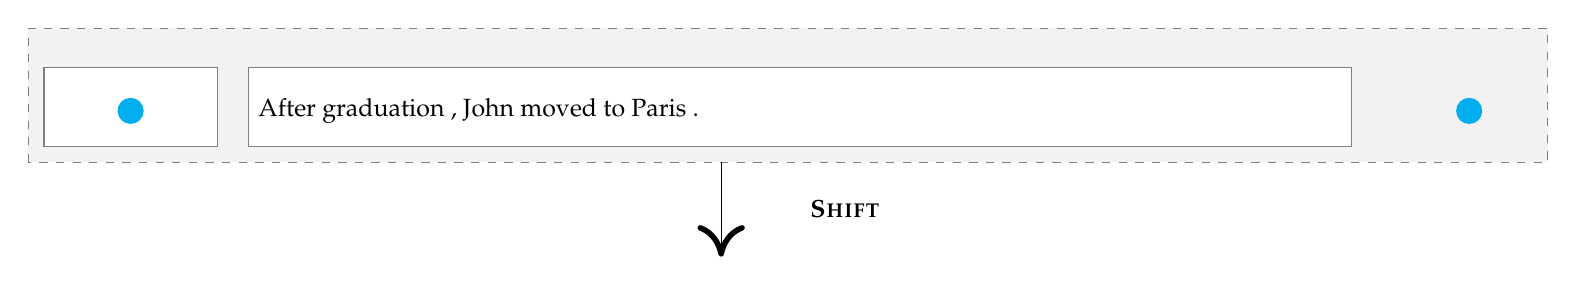
\begin{tikzpicture}[level distance=15mm, sibling distance=4cm, font=\small]
	\draw[color=gray,dashed,fill=lightgray!20] (.2,-.2) rectangle (19.5,1.5);
	\draw[color=gray,fill=white] (.4,0) rectangle (2.6,1);
	\node[fill=cyan, circle] at (1.5,.45) {};
	\draw[color=gray,fill=white] (3,0) rectangle (17,1);
	\node[anchor=west] at (3,.45) {After graduation , John moved to Paris .};
	\node[fill=cyan, circle] at (18.5,.45) {};
	\node[anchor=west] at (10,-.8) {\bf\small\textsc{Shift}};
	\draw[arrows={->[line width=2pt,length=4mm,width=6mm]}] (9,-.2) -- (9,-1.4);
	\end{tikzpicture}
	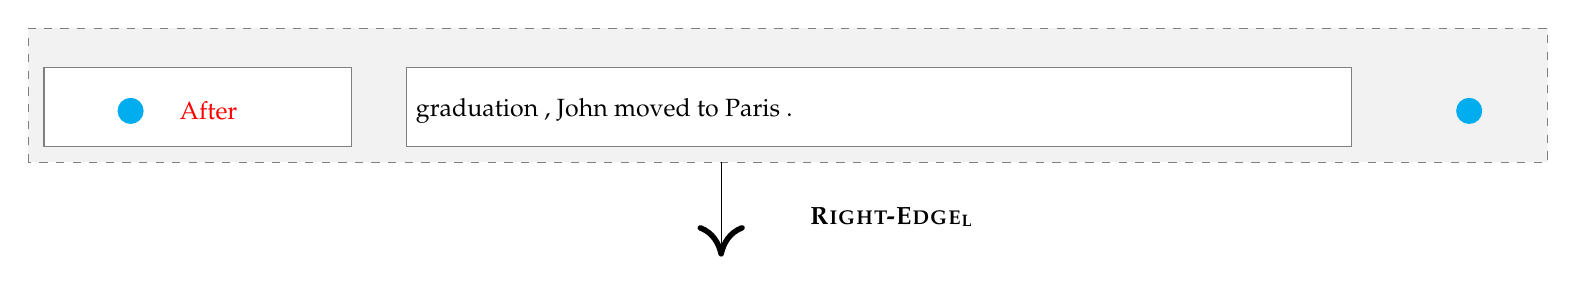
\begin{tikzpicture}[level distance=15mm, sibling distance=4cm, font=\small]
	\draw[color=gray,dashed,fill=lightgray!20] (.2,-.2) rectangle (19.5,1.5);
	\draw[color=gray,fill=white] (.4,0) rectangle (4.3,1);
	\node[fill=cyan, circle] at (1.5,.45) {};
	\node[color=red,anchor=west] at (2,.45) {After};
	\draw[color=gray,fill=white] (5,0) rectangle (17,1);
	\node[anchor=west] at (5,.45) {graduation , John moved to Paris .};
	\node[fill=cyan, circle] at (18.5,.45) {};
	\node[anchor=west] at (10,-.9) {\bf\small\textsc{Right-Edge\textsubscript L}};
	\draw[arrows={->[line width=2pt,length=4mm,width=6mm]}] (9,-.2) -- (9,-1.4);
	\end{tikzpicture}
	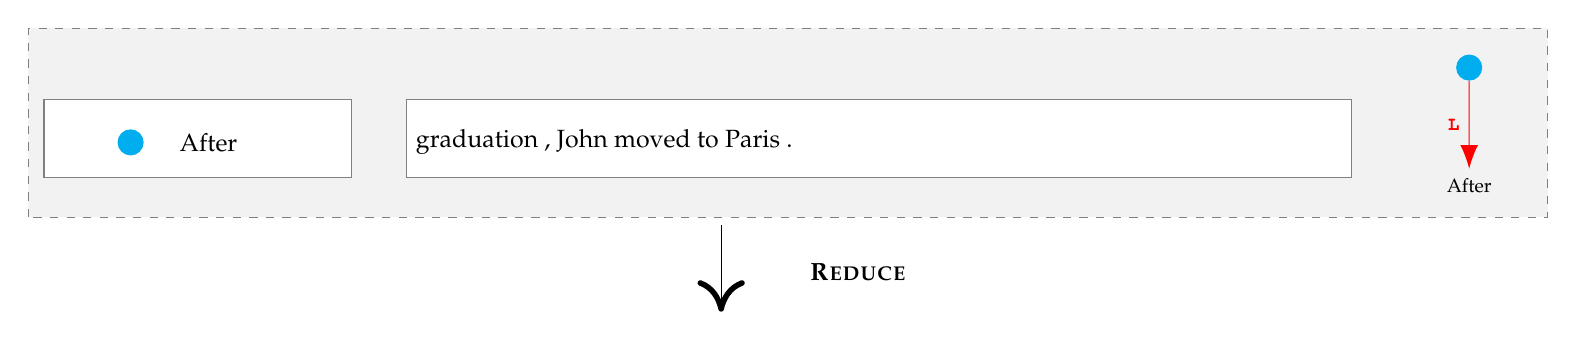
\begin{tikzpicture}[level distance=15mm, sibling distance=4cm, font=\small, -{Latex[length=3mm]}]
	\draw[color=gray,dashed,fill=lightgray!20] (.2,-.5) rectangle (19.5,1.9);
	\draw[color=gray,fill=white] (.4,0) rectangle (4.3,1);
	\node[fill=cyan, circle] at (1.5,.45) {};
	\node[anchor=west] at (2,.45) {After};
	\draw[color=gray,fill=white] (5,0) rectangle (17,1);
	\node[anchor=west] at (5,.45) {graduation , John moved to Paris .};
	\node[fill=cyan, circle] at (18.5,1.4) {}
	  child {node[font=\scriptsize] {After} edge from parent [red] node[font=\scriptsize\bf\ttfamily,left] {L}};
	\node[anchor=west] at (10,-1.2) {\bf\small\textsc{Reduce}};
	\draw[arrows={->[line width=2pt,length=4mm,width=6mm]}] (9,-.6) -- (9,-1.7);
	\end{tikzpicture}
	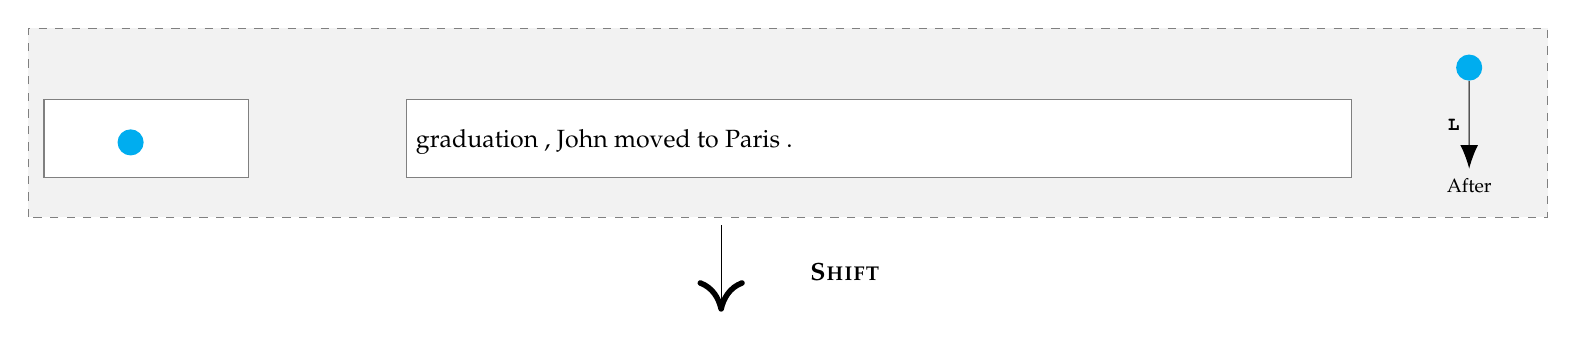
\begin{tikzpicture}[level distance=15mm, sibling distance=4cm, font=\small, -{Latex[length=3mm]}]
	\draw[color=gray,dashed,fill=lightgray!20] (.2,-.5) rectangle (19.5,1.9);
	\draw[color=gray,fill=white] (.4,0) rectangle (3,1);
	\node[fill=cyan, circle] at (1.5,.45) {};
	\draw[color=gray,fill=white] (5,0) rectangle (17,1);
	\node[anchor=west] at (5,.45) {graduation , John moved to Paris .};
	\node[fill=cyan, circle] at (18.5,1.4) {}
	  child {node[font=\scriptsize] {After} edge from parent node[font=\scriptsize\bf\ttfamily,left] {L}};
	\node[anchor=west] at (10,-1.2) {\bf\small\textsc{Shift}};
	\draw[arrows={->[line width=2pt,length=4mm,width=6mm]}] (9,-.6) -- (9,-1.7);
	\end{tikzpicture}
	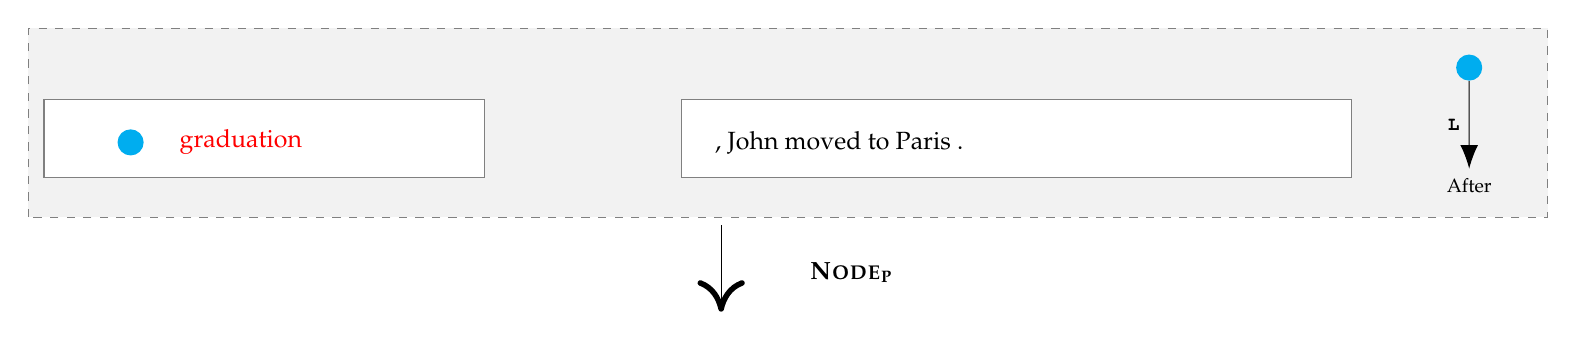
\begin{tikzpicture}[level distance=15mm, sibling distance=4cm, font=\small, -{Latex[length=3mm]}]
	\draw[color=gray,dashed,fill=lightgray!20] (.2,-.5) rectangle (19.5,1.9);
	\draw[color=gray,fill=white] (.4,0) rectangle (6,1);
	\node[fill=cyan, circle] at (1.5,.45) {};
	\node[color=red,anchor=west] at (2,.45) {graduation};
	\draw[color=gray,fill=white] (8.5,0) rectangle (17,1);
	\node[anchor=west] at (8.8,.45) {, John moved to Paris .};
	\node[fill=cyan, circle] at (18.5,1.4) {}
	  child {node[font=\scriptsize] {After} edge from parent node[font=\scriptsize\bf\ttfamily,left] {L}};
	\node[anchor=west] at (10,-1.2) {\bf\small\textsc{Node\textsubscript P}};
	\draw[arrows={->[line width=2pt,length=4mm,width=6mm]}] (9,-.6) -- (9,-1.7);
	\end{tikzpicture}
	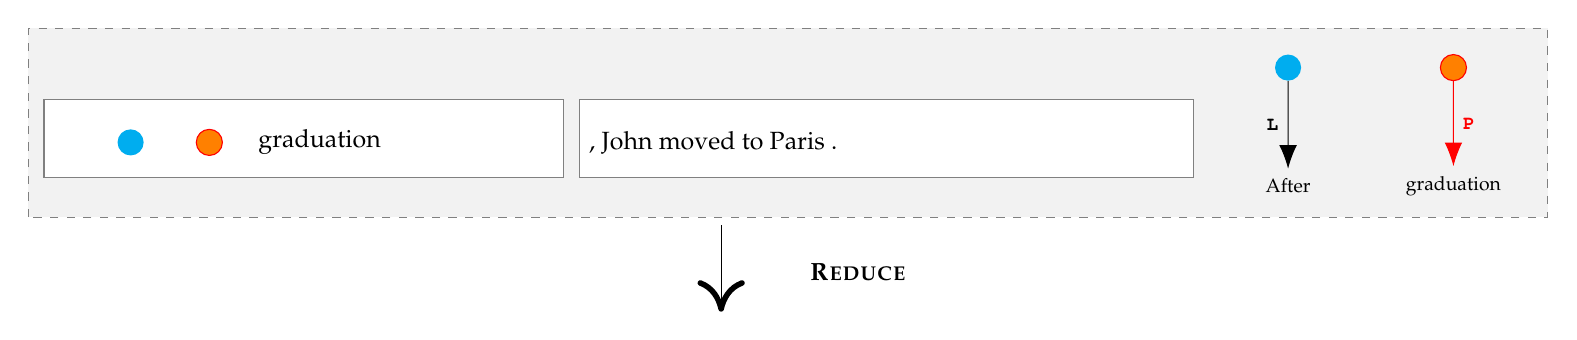
\begin{tikzpicture}[level distance=15mm, sibling distance=4cm, font=\small, -{Latex[length=3mm]}]
	\draw[color=gray,dashed,fill=lightgray!20] (.2,-.5) rectangle (19.5,1.9);
	\draw[color=gray,fill=white] (.4,0) rectangle (7,1);
	\node[fill=cyan, circle] at (1.5,.45) {};
	\node[fill=orange, draw=red, circle] at (2.5,.45) {};
	\node[anchor=west] at (3,.45) {graduation};
	\draw[color=gray,fill=white] (7.2,0) rectangle (15,1);
	\node[anchor=west] at (7.2,.45) {, John moved to Paris .};
	\node[fill=cyan, circle] at (16.2,1.4) {}
	  child {node[font=\scriptsize] {After} edge from parent node[font=\scriptsize\bf\ttfamily,left] {L}};
	\node[fill=orange, draw=red, circle] at (18.3,1.4) {}
	  child {node[font=\scriptsize] {graduation} edge from parent [red] node[font=\scriptsize\bf\ttfamily,right] {P}};
	\node[anchor=west] at (10,-1.2) {\bf\small\textsc{Reduce}};
	\draw[arrows={->[line width=2pt,length=4mm,width=6mm]}] (9,-.6) -- (9,-1.7);
	\end{tikzpicture}
\end{minipage}
\hspace{1cm}
\begin{minipage}{.4\columnwidth}
	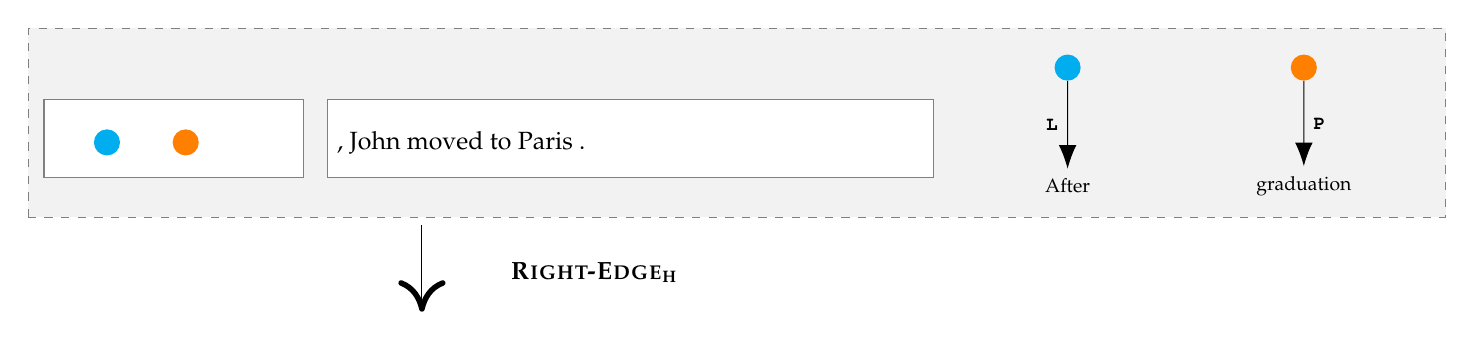
\begin{tikzpicture}[level distance=15mm, sibling distance=4cm, font=\small, -{Latex[length=3mm]}]
	\draw[color=gray,dashed,fill=lightgray!20] (0,-.5) rectangle (18,1.9);
	\draw[color=gray,fill=white] (0.2,0) rectangle (3.5,1);
	\node[fill=cyan, circle] at (1,.45) {};
	\node[fill=orange, circle] at (2,.45) {};
	\draw[color=gray,fill=white] (3.8,0) rectangle (11.5,1);
	\node[anchor=west] at (3.8,.45) {, John moved to Paris .};
	\node[fill=cyan, circle] at (13.2,1.4) {}
	  child {node[font=\scriptsize] {After} edge from parent node[font=\scriptsize\bf\ttfamily,left] {L}};
	\node[fill=orange, circle] at (16.2,1.4) {}
	  child {node[font=\scriptsize] {graduation} edge from parent node[font=\scriptsize\bf\ttfamily,right] {P}};
	\node[anchor=west] at (6,-1.2) {\bf\small\textsc{Right-Edge\textsubscript H}};
	\draw[arrows={->[line width=2pt,length=4mm,width=6mm]}] (5,-.6) -- (5,-1.7);
	\end{tikzpicture}
	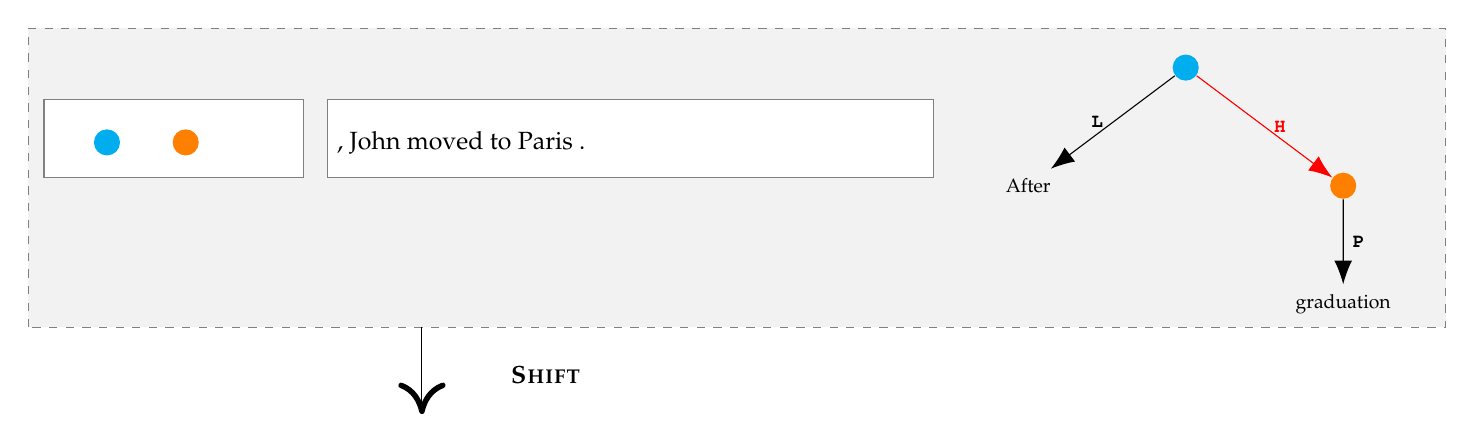
\begin{tikzpicture}[level distance=15mm, sibling distance=4cm, font=\small, -{Latex[length=3mm]}]
	\draw[color=gray,dashed,fill=lightgray!20] (0,-1.9) rectangle (18,1.9);
	\draw[color=gray,fill=white] (0.2,0) rectangle (3.5,1);
	\node[fill=cyan, circle] at (1,.45) {};
	\node[fill=orange, circle] at (2,.45) {};
	\draw[color=gray,fill=white] (3.8,0) rectangle (11.5,1);
	\node[anchor=west] at (3.8,.45) {, John moved to Paris .};
	\node[fill=cyan, circle] at (14.7,1.4) {}
	  child {node[font=\scriptsize] {After} edge from parent node[font=\scriptsize\bf\ttfamily,left] {L}}
	  child {node [fill=orange, circle] {}
	  {
	    child {node[font=\scriptsize] {graduation} edge from parent [black] node[font=\scriptsize\bf\ttfamily,right] {P}}
	  } edge from parent [red] node[font=\scriptsize\bf\ttfamily,right] {H} };
	\node[anchor=west] at (6,-2.5) {\bf\small\textsc{Shift}};
	\draw[arrows={->[line width=2pt,length=4mm,width=6mm]}] (5,-1.9) -- (5,-3);
	\end{tikzpicture}
	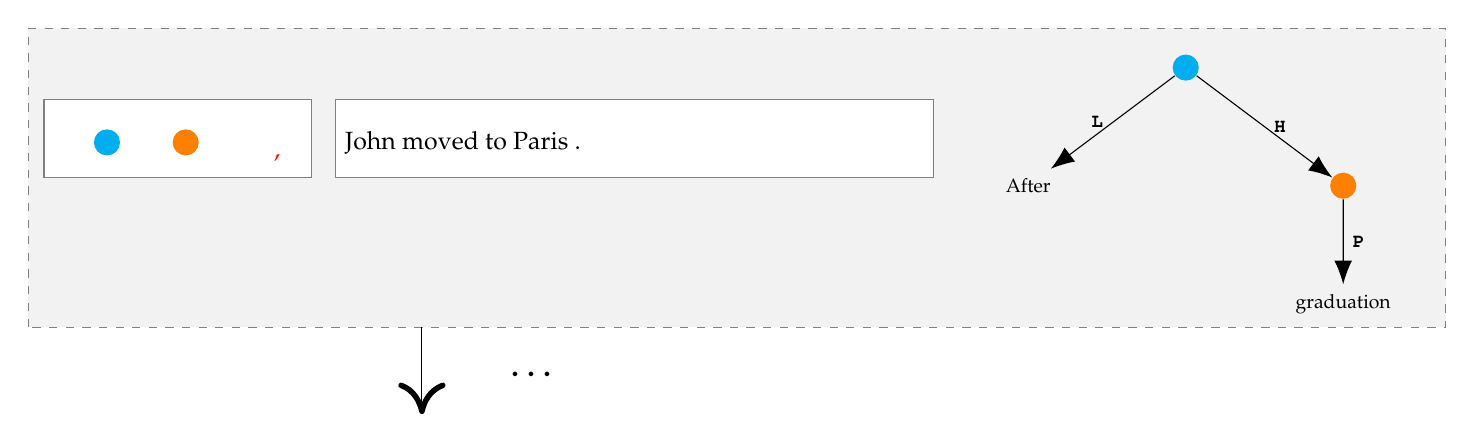
\begin{tikzpicture}[level distance=15mm, sibling distance=4cm, font=\small, -{Latex[length=3mm]}]
	\draw[color=gray,dashed,fill=lightgray!20] (0,-1.9) rectangle (18,1.9);
	\draw[color=gray,fill=white] (0.2,0) rectangle (3.6,1);
	\node[fill=cyan, circle] at (1,.45) {};
	\node[fill=orange, circle] at (2,.45) {};
	\node[color=red, anchor=west] at (3,.25) {,};
	\draw[color=gray,fill=white] (3.9,0) rectangle (11.5,1);
	\node[anchor=west] at (3.9,.45) {John moved to Paris .};
	\node[fill=cyan, circle] at (14.7,1.4) {}
	  child {node[font=\scriptsize] {After} edge from parent node[font=\scriptsize\bf\ttfamily,left] {L}}
	  child {node [fill=orange, circle] {}
	  {
	    child {node[font=\scriptsize] {graduation} edge from parent node[font=\scriptsize\bf\ttfamily,right] {P}}
	  } edge from parent node[font=\scriptsize\bf\ttfamily,right] {H} };
	\node[anchor=west] at (6,-2.5) {\Large \ldots};
	\draw[arrows={->[line width=2pt,length=4mm,width=6mm]}] (5,-1.9) -- (5,-3);
	\end{tikzpicture}
	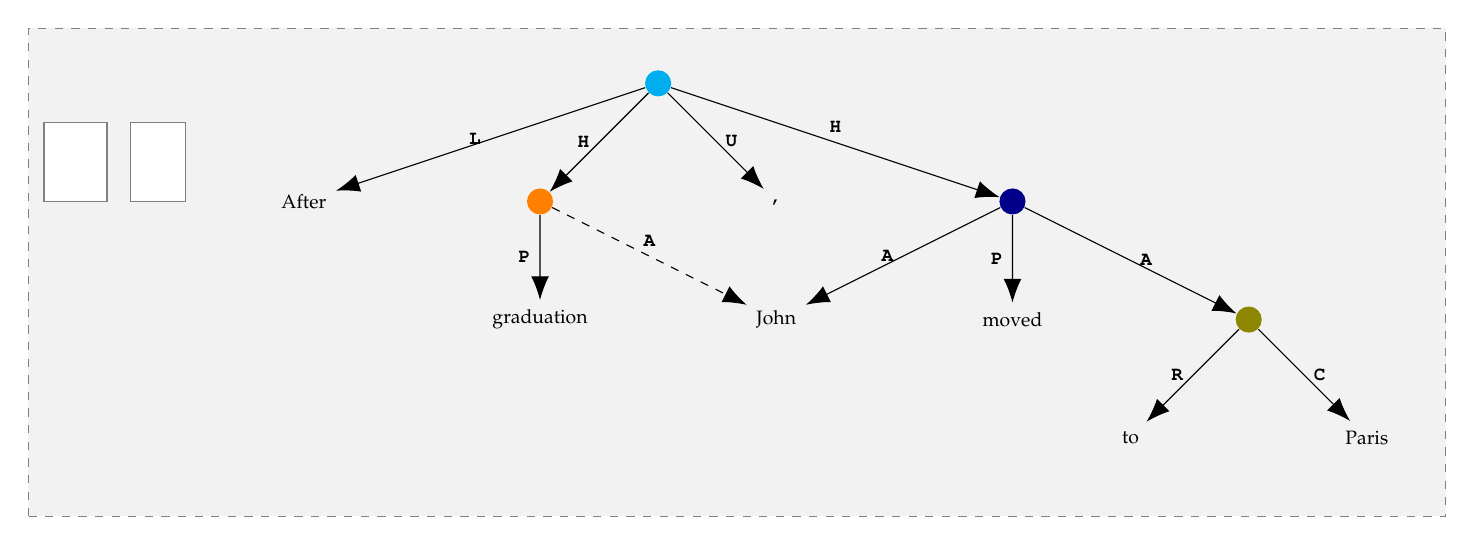
\begin{tikzpicture}[level distance=15mm, sibling distance=3cm, font=\small, -{Latex[length=3mm]}]
	\draw[color=gray,dashed,fill=lightgray!20] (0,-4) rectangle (18,2.2);
	\draw[color=gray,fill=white] (.2,0) rectangle (1,1);
	\draw[color=gray,fill=white] (1.3,0) rectangle (2,1);
    \node (ROOT) [fill=cyan,circle] at (8,1.5) {}
      child {node[font=\scriptsize] (After) {After} edge from parent node[font=\scriptsize\bf\ttfamily,left] {L}}
      child {node (graduation) [fill=orange,circle] {}
      {
        child {node[font=\scriptsize] {graduation} edge from parent node[font=\scriptsize\bf\ttfamily,left] {P}}
      } edge from parent node[font=\scriptsize\bf\ttfamily,left] {H} }
      child {node[font=\scriptsize\bf\ttfamily] {,} edge from parent node[font=\scriptsize\bf\ttfamily,right] {U}}
      child {node (moved) [fill=DarkBlue,circle] {}
      {
        child {node[font=\scriptsize] (John) {John} edge from parent node[font=\scriptsize\bf\ttfamily,left] {A}}
        child {node[font=\scriptsize] {moved} edge from parent node[font=\scriptsize\bf\ttfamily,left] {P}}
        child {node [fill=olive,circle] {}
        {
          child {node[font=\scriptsize] {to} edge from parent node[font=\scriptsize\bf\ttfamily,left] {R}}
          child {node[font=\scriptsize] {Paris} edge from parent node[font=\scriptsize\bf\ttfamily,right] {C}}
        } edge from parent node[font=\scriptsize\bf\ttfamily,right] {A} }
      } edge from parent node[font=\scriptsize\bf\ttfamily,above] {H} }
      ;
    \draw[dashed] (graduation) to node [font=\scriptsize\bf\ttfamily,above] {A} (John);
	\end{tikzpicture}
\end{minipage}
}

A \textbf{classifier} selects the next transition, given the current state's features.
Architecture: bidirectional LSTM RNN to encode text token features +
feedforward NN for classification.
For training, TUPA uses an oracle, returning correct transitions given gold-standard graphs.

\vfill

\section*{Multitask Architecture}

We use a \textbf{task-specific} BiLSTM for each task +
BiLSTM \textbf{shared} across all tasks.
We concatenate their outputs and select each transition using
a task-specific feedforward NN.
\begin{center}
   \vspace{-1mm}
   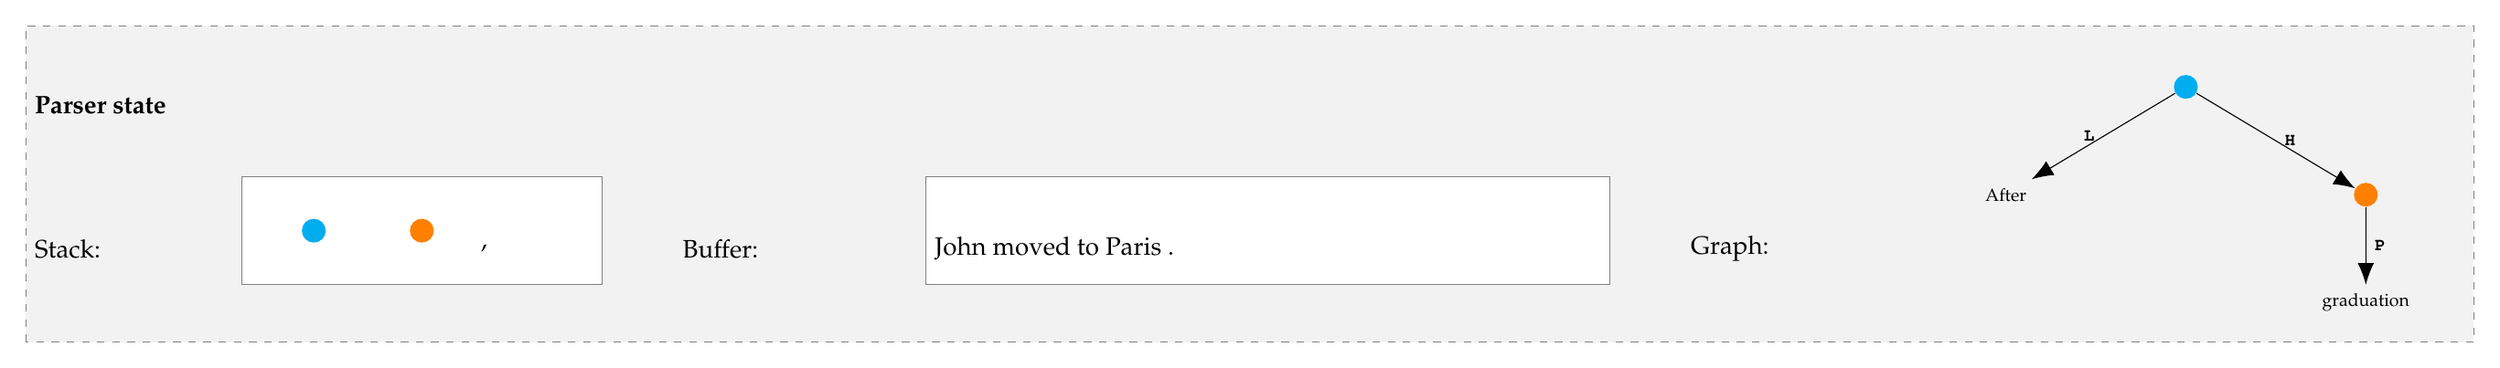
\begin{tikzpicture}[-{Latex[length=3mm]},level distance=15mm, sibling distance=5cm]
   \draw[color=gray,dashed,fill=lightgray!20] (0,-.8) rectangle (34,3.6);
   \node[anchor=west] at (0,2.5) {\textbf{Parser state}};
   \node[anchor=west] at (0,.5) {Stack:};
   \draw[color=gray,fill=white] (3,0) rectangle (8,1.5);
   \node[fill=cyan, circle] at (4,.75) {};
   \node[fill=orange, circle] at (5.5,.75) {};
   \node[anchor=west] at (6.2,.5) {,};
   \node[anchor=west] at (9,.5) {Buffer:};
   \draw[color=gray,fill=white] (12.5,0) rectangle (22,1.5);
   \node[anchor=west] at (12.5,.5) {John moved to Paris .};
   \node[anchor=west] at (23,.5) {Graph:};
   \node[fill=cyan, circle] at (30,2.75) {}
     child {node[font=\scriptsize] {After} edge from parent node[font=\scriptsize\bf\ttfamily,left] {L}}
     child {node [fill=orange, circle] {}
     {
       child {node[font=\scriptsize] {graduation} edge from parent node[font=\scriptsize\bf\ttfamily,right] {P}}
     } edge from parent node[font=\scriptsize\bf\ttfamily,right] {H} };
   \end{tikzpicture}
   
   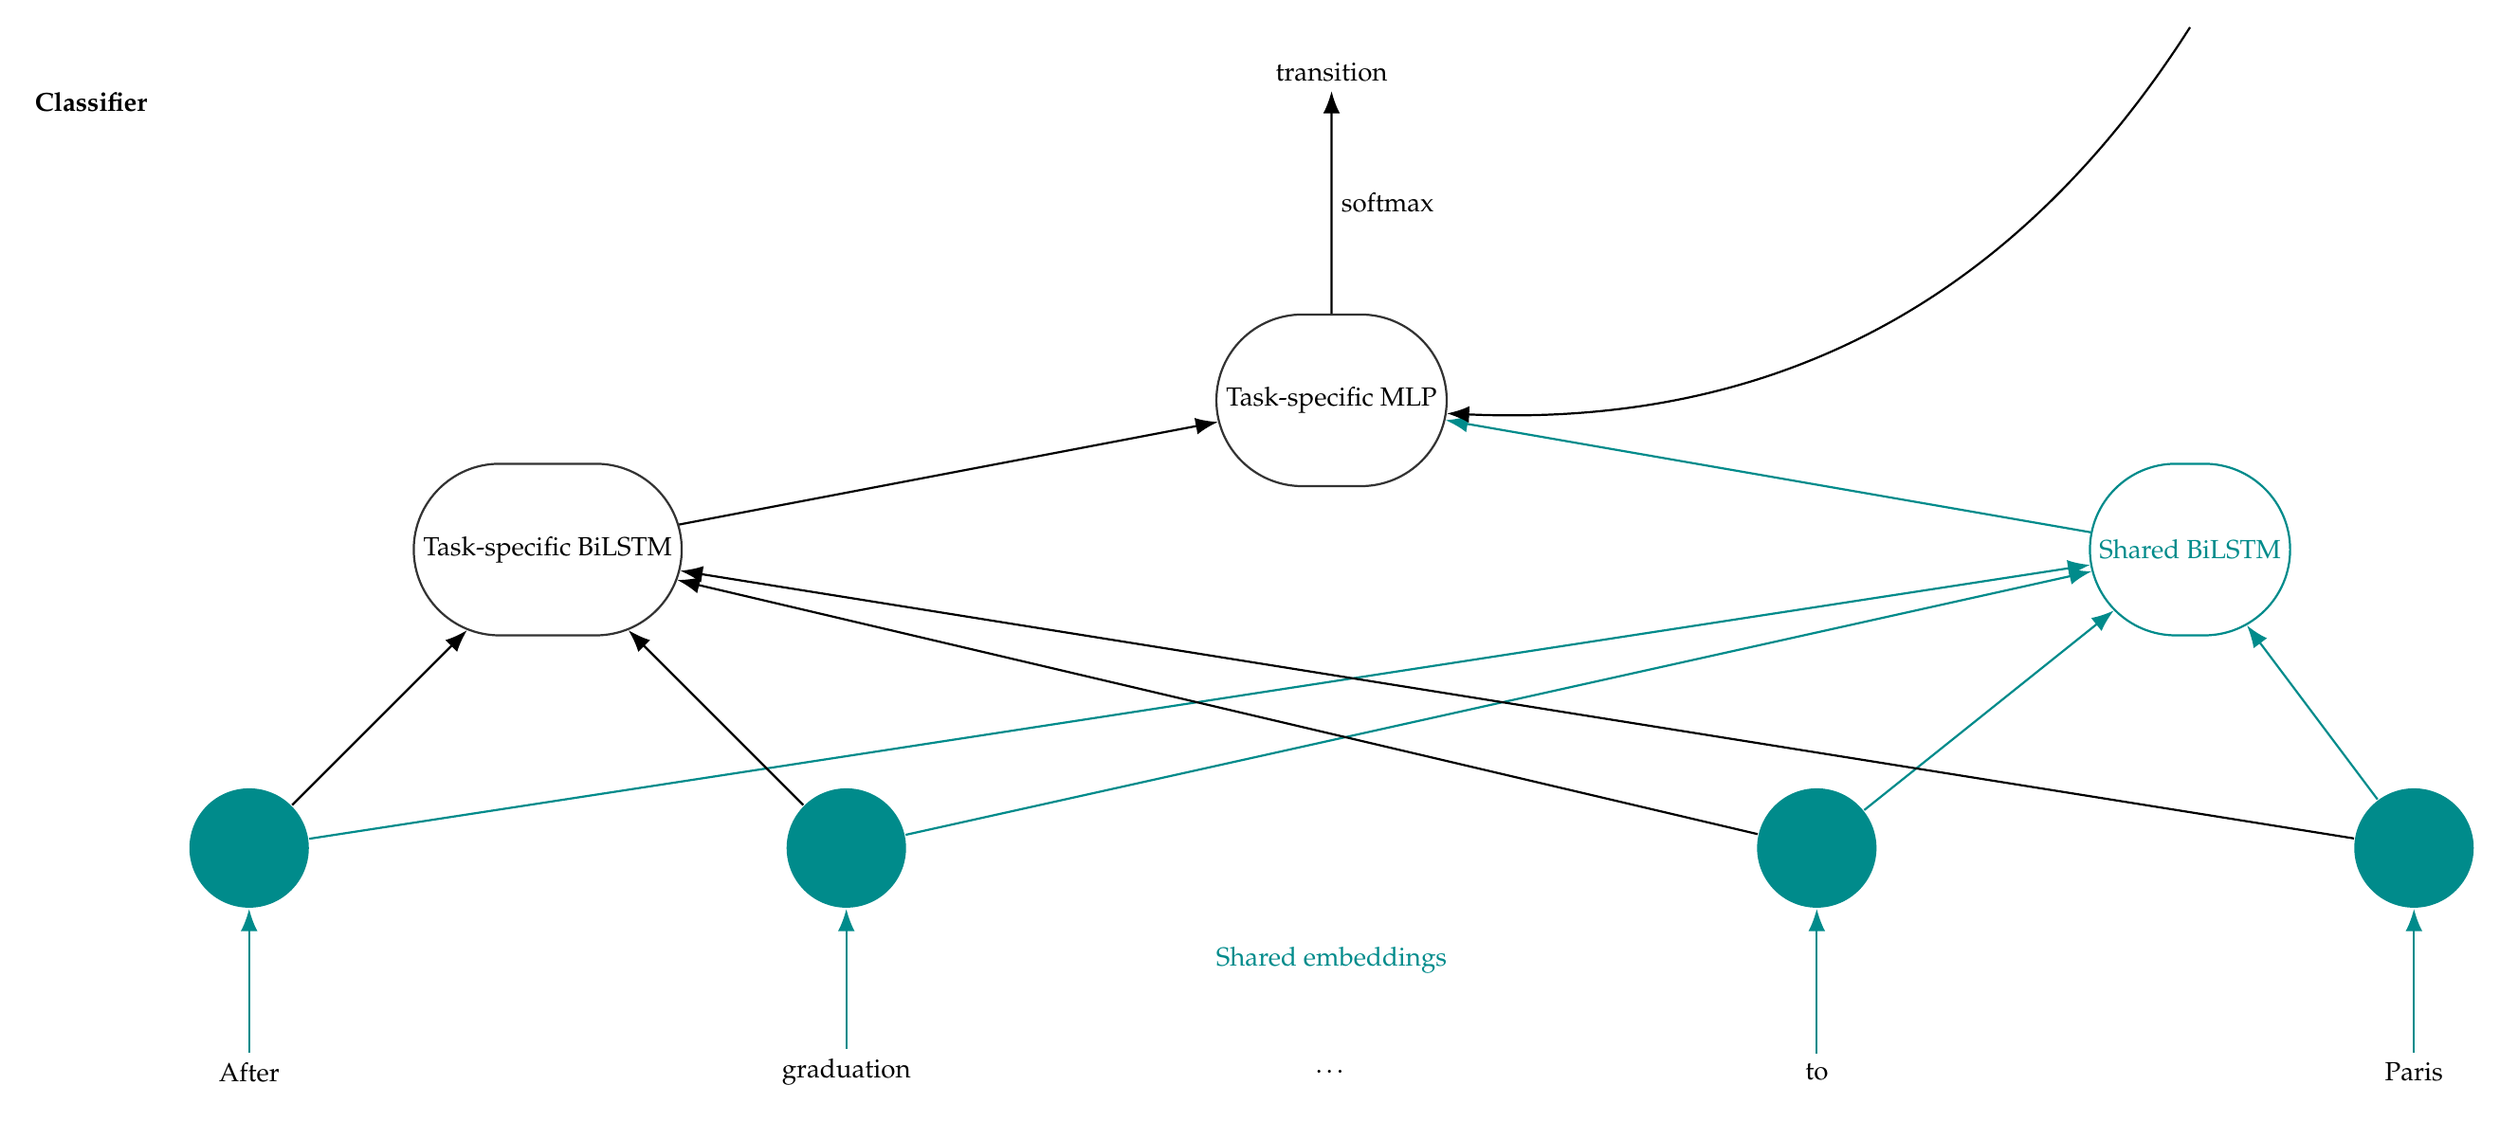
\begin{tikzpicture}[-{Latex[length=3mm]},thick]
   \node[anchor=west] at (-7,16) {\textbf{Classifier}};
   \tikzstyle{main}=[rounded rectangle, minimum size=23mm, draw=black!80, node distance=12mm]
   \node[main] (specific) at (0,10) {Task-specific BiLSTM};
   \node[main,color=DarkCyan] (shared) at (22,10) {Shared BiLSTM};
   \node[color=DarkCyan] (embeddings) at (10.5,4.5) {Shared embeddings};
   \foreach \i/\word in {-4/{After},4/{graduation},17/{to},25/{Paris}} {
       \node (x\i) at (\i,3) {\word};
       \node[main, minimum size=16mm, fill=DarkCyan, draw=none] (e\i) at (\i,6) {};
       \path[color=DarkCyan] (x\i) edge (e\i);
       \path (e\i) edge (specific);
       \path[color=DarkCyan] (e\i) edge (shared);
   }
    \node (x4) at (10.5,3) {\ldots};
    \node[main] (mlp) at (10.5,12) {Task-specific MLP};
    \path (specific) edge (mlp);
    \path[color=DarkCyan] (shared) edge (mlp);
    \coordinate (state) at (22,17);
    \path (state) edge [bend left] (mlp);
    \node (transition) at (10.5,16.4) {transition};
    \path (mlp) edge node[right] {softmax} (transition);
   \end{tikzpicture}
\end{center}

Limited capacity promotes generalization by using the shared parameters for all tasks
\cite{E17-1005}.

\hrule

\section*{Unified DAG Format}

We convert all representations into a format similar to UCCA and
supported by TUPA.

\begin{minipage}{.4\columnwidth}
  \begin{center}
  \begin{tikzpicture}[level distance=6cm, -{Latex[length=5mm]}, color=DarkGreen,
      every node/.append style={sloped,anchor=south,auto=false,font=\scriptsize\bf\ttfamily},
      level 1/.style={sibling distance=53mm},
      level 2/.style={sibling distance=3cm},
      level 3/.style={sibling distance=3cm}]
    \tikzstyle{word} = [font=\rmfamily,color=black]
    \node (ROOT) [word] {moved}
      child {node [word] {After}
      {
            child {node (graduation) [word] {graduation} edge from parent node {op} }
      } edge from parent node {time} }
      child {node (John) [fill=DarkGreen,circle] {}
      {
        child {node [word] {John} edge from parent node {name} }
      } edge from parent node {ARG0} }
      child {node [fill=DarkGreen,circle] {}
      {
        child {node [word] {Paris} edge from parent node {name} }
      } edge from parent node {ARG2} }
      ;
      \draw[dashed] (graduation) to node {ARG0} (John);
  \end{tikzpicture}
  \captionof{figure}{\color{DarkGreen} Converted AMR.}
  \end{center}
\end{minipage}
\hfill
\begin{minipage}{.6\columnwidth}
  \begin{center}
  \scalebox{.9}{
  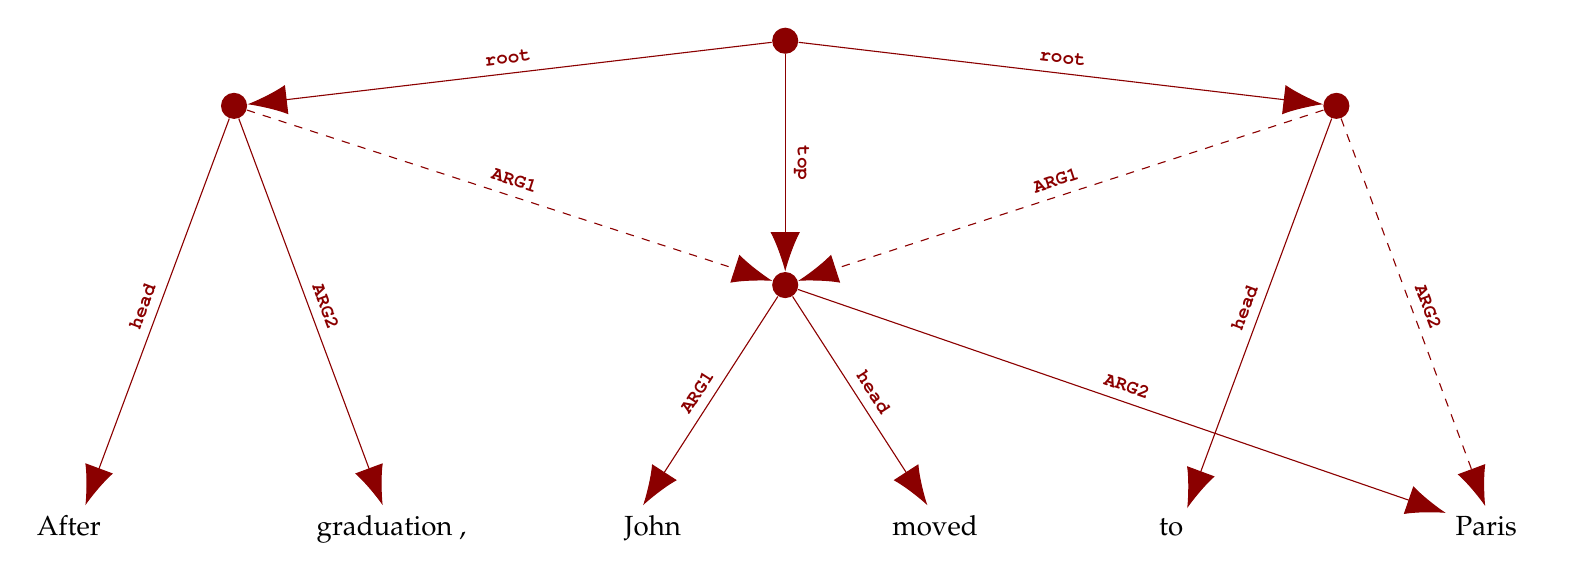
\begin{tikzpicture}[-{Latex[length=5mm]}, color=DarkRed,
      every node/.append style={sloped,anchor=south,auto=false,font=\scriptsize\bf\ttfamily},
      level 1/.style={sibling distance=7cm,level distance=1cm},
      level 2/.style={sibling distance=4cm,level distance=24mm},
      level 3/.style={level distance=34mm}]
    \tikzstyle{word} = [font=\rmfamily,color=black]
    \node (ROOT) [fill=DarkRed,circle] {}
      child {node (after) [fill=DarkRed,circle] {}
      {
        child {node [draw=none] {}
        {
          child {node [word] (after_word) {After{\color{white}g}} edge from parent [draw=none]}
        } edge from parent [draw=none] }
        child {node [draw=none] {}
        {
          child {node [word] (graduation) {graduation ,} edge from parent [draw=none]}
        } edge from parent [draw=none] }
      } edge from parent node {root}}
      child {node [draw=none] {}
      {
        child {node (moved) [fill=DarkRed,circle] {}
        {
          child {node [word] {\quad{\color{white}g} John} edge from parent node {ARG1}}
          child {node [word] {moved{\color{white}g}} edge from parent node {head}}
        } edge from parent [draw=none] }
      } edge from parent [draw=none] }
      child {node (to) [fill=DarkRed,circle] {}
      {
        child {node [draw=none] {}
        {
            child {node [word] (to_word) {to{\color{white}g}} edge from parent [draw=none]}
          } edge from parent [draw=none] }
          child {node [draw=none] {}
        {
          child {node [word] (Paris) {Paris{\color{white}g}} edge from parent [draw=none]}
        } edge from parent [draw=none] }
      } edge from parent node {root}}
      ;
      \draw (ROOT) to node {top} (moved);
      \draw (after) to node {head} (after_word);
      \draw (after) to node {ARG2} (graduation);
      \draw[dashed] (after) to node {ARG1} (moved);
      \draw[dashed] (to) to node {ARG1} (moved);
      \draw (to) to node {head} (to_word);
      \draw (moved) to node {ARG2} (Paris);
      \draw[dashed] (to) to node {ARG2} (Paris);
  \end{tikzpicture}}
  \captionof{figure}{\color{DarkRed} Converted DM.}
  \scalebox{.9}{
  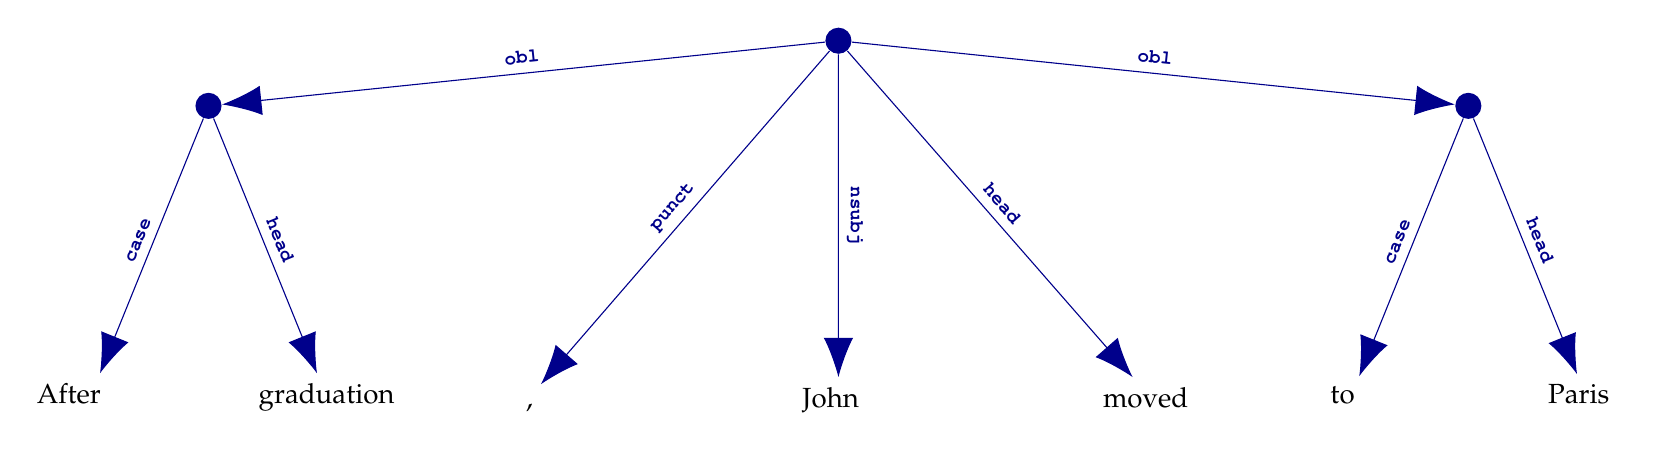
\begin{tikzpicture}[-{Latex[length=5mm]}, color=DarkBlue,
      every node/.append style={sloped,anchor=south,auto=false,font=\scriptsize\bf\ttfamily},
      level 1/.style={sibling distance=4cm,level distance=1cm},
      level 2/.style={sibling distance=3cm,level distance=4cm}]
    \tikzstyle{word} = [font=\rmfamily,color=black]
    \node (ROOT) [fill=DarkBlue,circle] {}
      child {node (after) [fill=DarkBlue,circle] {}
      {
        child {node [word] {After{\color{white}g}\quad\quad} edge from parent node {case}}
        child {node [word] {\quad graduation\quad\quad} edge from parent node {head}}
      } edge from parent node {obl}}
      child {node {}
      {
        child {node [word] (comma) {\quad,{\color{white}g}} edge from parent [draw=none]}
      } edge from parent [draw=none]}
      child {node {}
      {
        child {node [word] (John) {John{\color{white}g}} edge from parent [draw=none]}
      } edge from parent [draw=none]}
      child {node {}
      {
        child {node [word] (moved) {moved{\color{white}g}} edge from parent [draw=none]}
      } edge from parent [draw=none]}
      child {node (to) [fill=DarkBlue,circle] {}
      {
          child {node [word] {to{\color{white}g}} edge from parent node {case}}
          child {node [word] {Paris{\color{white}g}} edge from parent node {head}}
      } edge from parent node {obl}}
      ;
      \draw (ROOT) to node {punct} (comma);
      \draw (ROOT) to node {nsubj} (John);
      \draw (ROOT) to node {head} (moved);
  \end{tikzpicture}}
  \captionof{figure}{\color{DarkBlue} Converted UD.}
  \end{center}
\end{minipage}

\hrule



\section*{Experiments}

In \textbf{English}, we train on the {\color{Indigo} UCCA Wiki} training set
(adding various tasks as auxiliaries), and test on the {\color{Indigo} 20K} out-of-domain test set.
In \textbf{French} and \textbf{German}, we train on the {\color{Indigo} 20K} training set
(using {\color{DarkBlue} UD} in the same language as auxiliary),
and test on the {\color{Indigo} 20K} test set.

\begin{center}
\vspace{-1cm}
\setlength\tabcolsep{1cm}
\begin{tabular}{l|lll|lll}
& \multicolumn{3}{c|}{\bf\small Primary} & \multicolumn{3}{c}{\bf\small Remote} \\
& \textbf{\small LP} & \textbf{\small LR} & \textbf{LF}
& \textbf{\small LP} & \textbf{\small LR} & \textbf{LF} \\
\hline
\bf English (out-of-domain) & \\
TUPA \cite{hershcovich2017a}
& 68.7 & 68.5 & \large 68.6 & 38.6 & 18.8 & \large 25.3 \\
Our single ({\color{Indigo} UCCA} only)
& 68.9 & 68.9 & \large 68.9 & 40.7 & 19.6 & \large 26.5 \\
\cline{1-1}
+ \color{DarkGreen} AMR
& 69.4 & 69.6 & \large 69.5 & 44.3 & 21.4 & \large 28.8 \\
+ \color{DarkRed} DM
& 70.1$\star$ & 69.5 & {\large 69.8}$\star$ & 40 & 18.6 & \large 25.4 \\
+ \color{DarkBlue} UD$^{++}$
& 69.8$\star$ & 69.4 & \large 69.6 & 39.8 & 14.7$\dagger$ & {\large 21.4}$\dagger$ \\
+ {\color{DarkGreen} AMR} + \color{DarkRed} DM
& 69.8$\star$ & 69.5 & {\large 69.7}$\star$ & 48.8$\star$ & 19.6 & \large 28 \\
+ {\color{DarkGreen} AMR} + \color{DarkBlue} UD$^{++}$
& 69.7$\star$ & 70$\star$ & {\large 69.8}$\star$ & 39 & 21.4 & \large 27.6 \\
+ {\color{DarkRed} DM} + \color{DarkBlue} UD$^{++}$
& 70$\star$ & 68.9 & \large 69.4 & 47.4$\star$ & 22 & {\large 30}$\star$ \\
+ {\color{DarkGreen} AMR} + {\color{DarkRed} DM} + \color{DarkBlue} UD$^{++}$
& 71$\star$ & 72.2$\star$ & {\large \textbf{71.6}}$\star$ & 43.9 & 24.8$\star$ & {\large \textbf{31.6}}$\star$ \\
\hline
\bf French (in-domain) & \\
Our single ({\color{Indigo} UCCA} only) & 64.1 & 60.6 & \large 62.3 & 20 & \enskip 5.7 & \enskip \large 8.8 \\
+ \color{DarkBlue} UD & 68.7$\star$ & 68.6$\star$ & {\large \textbf{68.6}}$\star$ & 15.8 & \enskip 5.7 & \enskip \large 8.3 \\
\hline
\bf German (in-domain) & \\
Our single ({\color{Indigo} UCCA} only) & 73.3 & 71.7 & \large 72.5 & 57.1 & 17.7 & \large 27.1 \\
+ \color{DarkBlue} UD & 73.7$\star$ & 72.6$\star$ & {\large \textbf{73.2}}$\star$ & 61.8 & 24.9$\star$ & {\large \textbf{35.5}}$\star$
\end{tabular}
\captionof{table}{Labeled precision, recall and $F_1$ (in~\%) for primary and remote edges
on the UCCA 20K gold standard test sets.
$\star$~indicates significantly better than \textit{Single},
and $\dagger$ significantly worse.}
\end{center}

Our basic single-task model slightly outperforms the TUPA baseline, due to more features.
All multitask models further improve UCCA parsing. The contribution is largely additive.

\hrule


\section*{Conclusion}

We propose a unified DAG format for semantic representation,
and train a transition-based semantic DAG parser in a multitask setting.
We demonstrate that multitask learning improves UCCA parsing in out-of-domain settings
or when training data is scarce or noisy,
using unlabeled AMR, SDP and UD parsing as auxiliaries.\footnote{Code:
\url{http://github.com/danielhers/tupa} \hfill
Corpora: \url{http://github.com/huji-nlp/ucca-corpora} \hfill
Implemented using DyNet: \url{http://github.com/clab/dynet}}

A natural question is whether our method can benefit AMR, SDP or UD.
Future work will investigate whether a single
algorithm and architecture can be competitive on all of these.
\vspace{-5mm}

\begin{multicols}{2}
\color{DarkSlateGray}
\tiny\titleformat*{\section}{\small}
\bibliographystyle{plain}
\bibliography{references}
\end{multicols}

\end{multicols}
\end{document}
